\section{Experiment 3: EVS Resampling Study}

In the third experiment, we performed a resampling study based on the EVS data to assess
how the result obtained for Experiments 1 and 2 carried over to real data applications.
EVS is a large-scale, cross-national survey on human values administered in around 50 countries
across Europe.
It covers a wide range of human values regarding family, work, environment, perceptions of 
life, politics, society, religion, morality, and national identity.
It is a high-quality survey widely used for comparative studies between European countries.
Furthermore, it is accessible free of charge and it represents the type of data social scientist 
regularly analyse.
Variables in the EVS data are discrete numerical and categorical items following a 
variety of distributions.

In Experiment 3, we considered the original EVS data as a population data for a resampling study.
We investigated the performance of the methods by resampling $S=1000$ datasets of $n$ units from this 
population.
For each replicate, we imposed missing values, treated them with the same methods used in 
experiments 1 and 2, and pooled the analysis model parameter estimates.
This procedure was repeated for a low-dimensional and a high-dimensional condition. 
As the number of predictors in the data was fixed ($p = 243$), the dimensionality of the data was 
controlled by defining different sizes for the sample taken from the EVS population data 
($n = (1000, 300)$).

\subsection{Resampling Study Procedure} \label{resProc}

\subsubsection{Data preparation and generation}
	We used the third prerelease of the 2017 wave of EVS data \citep{EVS:2017} to define a population dataset 
	with no missing values.
	The original dataset contained 55,000 observations from 34 countries.
	We selected only the four founding countries of the European Union included in the dataset (France, Germany,
	Italy, and the Netherlands) and excluded all columns of the data that were either duplicated
	information (recoded versions of other variables), or meta data (e.g. time of interview,
	mode of data collection).

	We run a single imputation predictive mean matching (PMM) algorithm to fill the originally missing values 
	and obtain a pseudo fully-observed dataset.
	This imputation step was completed using the $mice()$ imputation function in the mice R package.
	PMM was chosen for the task as it is a flexible imputation method that maintains the distributional 
	characteristics of the original data.
	Predictors for the imputation models were selected based on the variable selection procedure described in
	\citeauthor{vanBuurenEtAl:1999} (\citeyear[pp. 687–688]{vanBuurenEtAl:1999}) by using the \emph{quickpred()}
	R function and setting the minimum correlation threshold to 0.3.
	The number of MI iterations was set to 200.
	This imputation procedure was used to obtain a population dataset of pseudo-fully observed data, and 
	therefore it did not require multiple imputation itself.
	At the end of this data cleaning process, we obtained a fully observed dataset of 8,045 observations 
	($n$), across 4 countries, and 243 variables ($p$).
	For every $s$ replicate in the resampling study, a bootstrap sample was generated by sampling with 
	replacement $n$ observations from this data population.

\subsubsection{Analysis models}

	To define plausible analysis models, we searched for models that have been used in published articles
	testing social scientific theories on the EVS data.
	The search was performed by screening the repository of publications using EVS data available on the EVS 
	website \citep{EVSbib}.

	As a result, we defined two linear regression models, models 1 and 2, of the same form:
%	
	\begin{equation}
		y = \beta_{0} + \beta_{1} x + \bm{\beta} \bm{C}  \label{eqn:lm}
	\end{equation}
%
	where a dependent variable $y$ is regressed on a variable of interest $x$ and a set of control variables
	$\bm{C}$.
	In this scenario, $\beta_{1}$ is a focal parameter that a researcher wants to use to test some hypothesis.

	The first version of linear model \eqref{eqn:lm}, Model 1, was inspired by \cite{koneke:2014}:
	$y^{(1)}$, its dependent variable, was a 10-point EVS item measuring euthanasia acceptance 
	(`Can [euthanasia] always be justified, never be justified, or something in between?');
	the predictor of interest $x^{(1)}$ was a 4-point item measuring the self-reported importance of religion in 
	one's life;
	the matrix of covariates $\bm{C}^{(1)}$ included trust in the health care system, trust in the state, 
	trust in the press, country, sex, age, education, and religious denomination.
	This model represents a plausible analysis a researcher would perform to test a hypothesis regarding the 
	effect of religiosity on the acceptance of end-of-life treatments.

	Model 2, the second version of the linear model in equation \ref{eqn:lm}, was inspired by \cite{immerzeel:2015}.
	The dependent variable $y^{(2)}$ was an harmonized variable constructed by EVS to describe the respondents' 
	tendency to vote left or right-wing parties, expressed on a 10-point left-to-right continuum.
	The predictor of interest $x^{(2)}$ was a scale measuring respondents' attitudes toward immigrants and immigration 
	(`nativist attitudes scale').
	The scale was obtained by taking the average of respondents' agreement, on a scale from 1 to 10, with three 
	statements: `immigrants take jobs away from natives', `immigrants increase crime problems', and 
	`immigrants are a strain on welfare system'.
	The control variables used were: 
	attitudes toward law and order, attitudes toward authoritarianism, interest in politics, level of political activity,  
	country, sex, age, education, employment status, socio-economic status, importance of religion in life, 
	religious denomination, and the size of town where interview was conducted.
	A researcher might fit this model and look at the estimate and standard error of $\beta^{(2)}_{1}$, 
	the `nativist attitude' regression coefficient, to test an hypothesis regarding the effect of xenophobia on voting 
	tendencies.

\subsubsection{Missing data imposition}

	Missing data were imposed on six variables according to the same strategy described for experiments 1 and 2.
	The variables target of missing value imposition were the two dependent variables in models 1 and 2 (i.e., 
	euthanasia acceptance, and left-to-right voting tendency); 
	religiosity (the focal predictor and a control variable in models 1 and 2 respectively);
	and the three items making up the ``nativist attitudes'' scale (the focal predictor in the second model).

	The response model form was the same as in Equation \eqref{eqn:rm} and three variables were included in $\tilde{Z}$: 
	age, education, and an item measuring trust in new people. 
	Older people tend to have higher item non-response rates than younger people, and 
	lower educated people tend to have higher item non-response rates than higher educated people 
	\citep{guadagnoliCleary:1992, leeuwEtAl:2003}.
	We assumed that people with less trust in strangers have a higher item non-response tendency as 
	they are likely to withhold more information from the interviewer (a stranger).

\subsubsection{Imputation}
	
	Missing values were treated according to all the methods previously discussed.
	The imputation methods were parametrized as in Experiments 1 and 2, and
	convergence checks were performed in the same way.
	The imputation models were considered to have converged after 60 iterations.

\subsection{Results}

	When estimating multiple linear regressions, all partial regression coefficients are influenced by the 
	imputation of the dependent variable and a handful of predictors.
	Therefore, it is important to observe the estimation bias and CI coverage rates for all model parameters.
	Figure \ref{fig:exp4_bias_allP} reports the absolute values of the PRBs for the intercept and all the partial 
	regression coefficients in Model 2, under the different imputation methods, for both the low- and high-dimensional
	conditions.
	Figure \ref{fig:exp4_ci_allP} reports CIC results in the same way.
	Results for Model 1 are reported in the supplementary materials.

	Focusing first on the focal parameter $\beta_1$, most of the MI methods resulted in negligible biases ($| PRB | < 10\%$) 
	in both conditions.
	The two exceptions were bridge and MI-RF. 
	The former was very competitive in the low-dimensional condition but led to extreme bias and over-coverage in the 
	high-dimensional condition.
	The latter provided the largest focal $|\text{PRB}|$ among the other MI methods, and it was consistently 
	outperformed even by Complete Case analysis.
	Furthermore, they also provided the worst coverage performance for the focal regression coefficient.

	DURR, IURR and MI-PCA resulted in the lowest bias for the focal parameter in both conditions.
	They also resulted in non-significant deviations from nominal coverage in both the low and high
	dimensional conditions.
	While DURR and IURR resulted in slightly smaller PRB than MI-PCA, the latter resulted in the smallest 
	deviations from nominal coverage.

	Looking at all the estimated regression coefficients and intercept, even MI-OP did not provide entirely unbiased
	model estimation.
	Around half of the estimates obtained with MI-OP had large bias ($|PRB|>10\%$).
	The largest MI-OP bias was considerable: around 40\%, in the low dimensional condition, and 20\%, in the 
	high-dimensional one.
	In both the high- and low-dimensional conditions, DURR, IURR, blasso, MI-CART, and
	missForest showed only slightly larger PRBs than MI-OP.
	MI-PCA and MI-RF showed similar trends but presented larger PRBs above the 10\% threshold.
	Bridge demonstrated the same results described in the simulation studies. 
	It was a competitive method in low dimensional scenarios, but it was inadequate to deal with high-dimensional 
	data imputation (all but one PRB are larger than 50\%).
	For all the other methods, PRBs above the $10\%$ threshold were less extreme in the high-dimensional condition.

	DURR, IURR, and MI-CART maintained similar coverage patterns to MI-OP, with only 
	a few significant CICs deviations from nominal coverage rates.
	MI-PCA, blasso, and MI-RF over-covered more than half of the parameters.
	All MI methods led to CIC closer to nominal rates in the high-dimensional condition.
	
	As expected, imputation by missForest led to significant under-coverage of most regression coefficients, 
	including the focal parameter. 
	Despite showing poor performances in terms of bias, Complete Case analysis manifested good 
	coverage of all true parameter values.
	However, this was a result of the smaller sample size used for estimating the analysis model, rather than 
	a positive feature of the method.
	The smaller samples produced wider intervals which covered the true values even when the point-estimates 
	were biased.

\begin{figure}
	\centering
	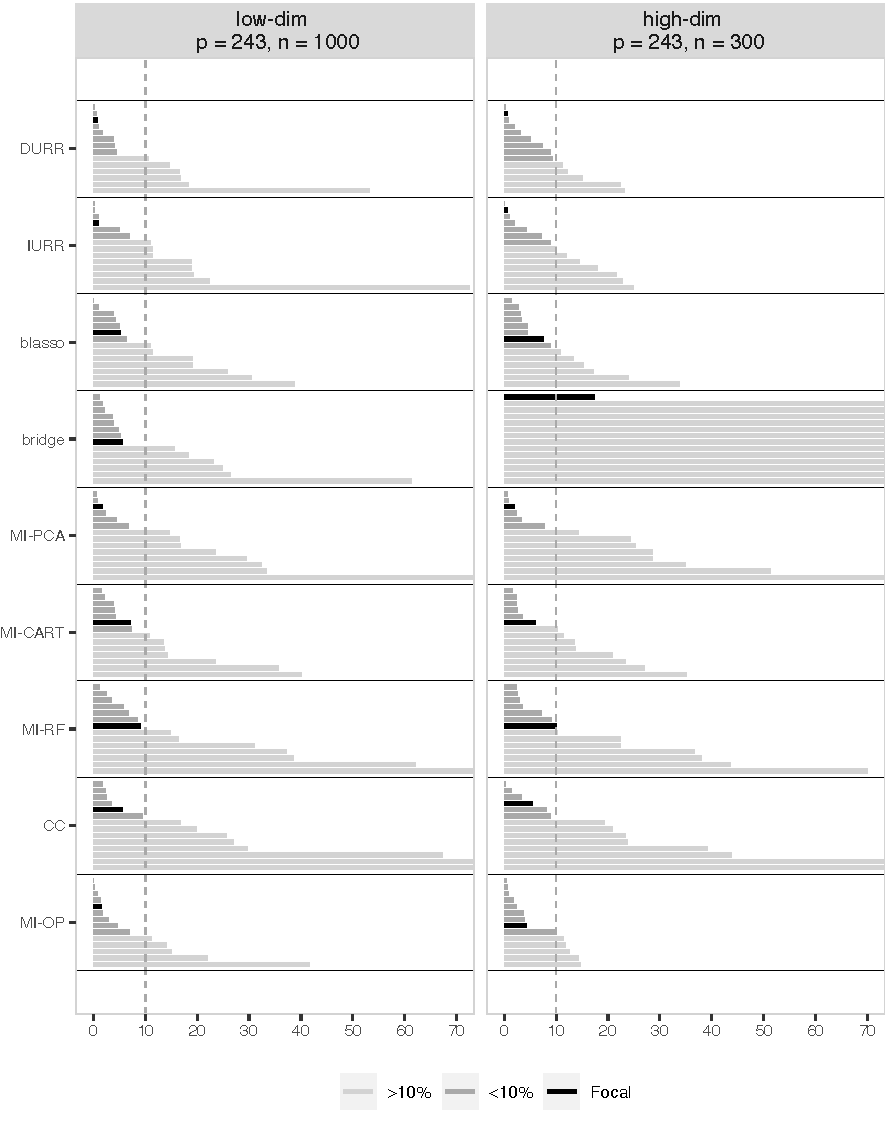
\includegraphics{\pathFIG/exp4_imp_bias_allParms_m2.pdf}
	\caption{
		$|\text{PRB}|$ for all the model parameters in model 2.
		For each method, the PRBs are reported by increasing absolute value.
		The $|\text{PRB}|$ for the focal parameter estimate is reported in black.
	}
		\label{fig:exp4_bias_allP}
\end{figure}

\begin{figure}
	\centering
	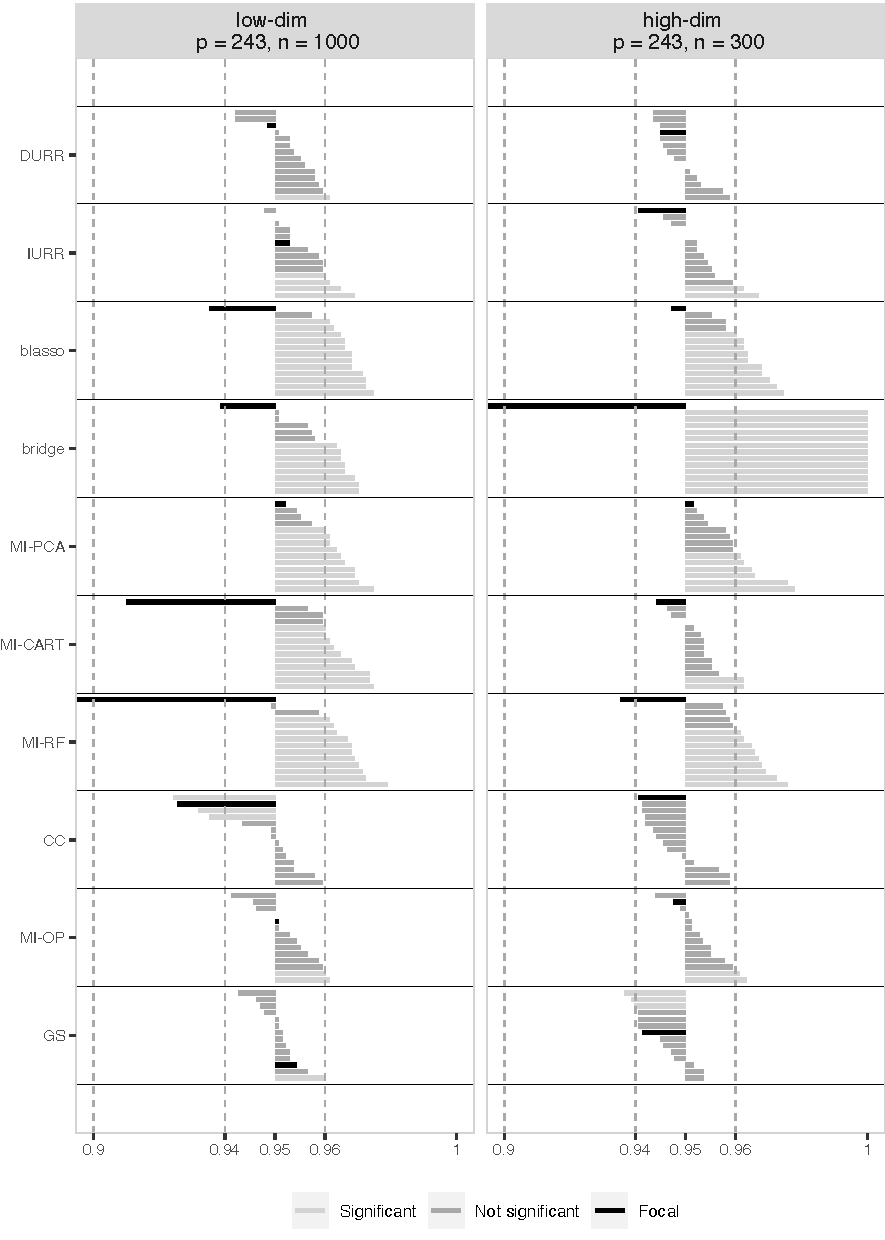
\includegraphics{\pathFIG/exp4_imp_ci_allParms_m2.pdf}
	\caption{
		CIC for all model parameter in model 2.
		For each method, the CICs are reported by increasing value.
		The CIC of the focal parameter is reported in black.
	}
	\label{fig:exp4_ci_allP}
\end{figure}

\FloatBarrier

\subsubsection{Imputation Time}

	Table \ref{tab:time} reports the average imputation time for the different methods.
	IURR and DURR were the most time-consuming methods with imputation times above the hour 
	in our low-dimensional conditions. 
	MI-PCA and blasso imputation had imputation times of a minute or less.
	In the high-dimensional condition, IURR and DURR were not as time-intensive due to the smaller
	sample size, but still required more than ten times the time of MI-PCA and blasso imputation.

\begin{table}
	\centering
	\begin{tabular}{l | r | r | r | r | r | r | r | r }
		condition & DURR & IURR & blasso & bridge & MI-PCA & MI-CART & MI-RF & MI-OP \\
		\hline
		1 & 73.20 & 75.90 & 1.40 & 8.10 & 0.60 & 4.00 & 11.30 & 2.20 \\ 
		2 & 6.10 & 9.70 & 0.50 & 3.20 & 0.40 & 1.40 & 4.70 & 1.90 	
	\end{tabular}
	\caption{\label{tab:time}Average imputation time in minutes.}
\end{table}

\FloatBarrier


